
%% bare_conf.tex
%% V1.3
%% 2007/01/11
%% by Michael Shell
%% See:
%% http://www.michaelshell.org/
%% for current contact information.
%%
%% This is a skeleton file demonstrating the use of IEEEtran.cls
%% (requires IEEEtran.cls version 1.7 or later) with an IEEE conference paper.
%%
%% Support sites:
%% http://www.michaelshell.org/tex/ieeetran/
%% http://www.ctan.org/tex-archive/macros/latex/contrib/IEEEtran/
%% and
%% http://www.ieee.org/

%%*************************************************************************
%% Legal Notice:
%% This code is offered as-is without any warranty either expressed or
%% implied; without even the implied warranty of MERCHANTABILITY or
%% FITNESS FOR A PARTICULAR PURPOSE! 
%% User assumes all risk.
%% In no event shall IEEE or any contributor to this code be liable for
%% any damages or losses, including, but not limited to, incidental,
%% consequential, or any other damages, resulting from the use or misuse
%% of any information contained here.
%%
%% All comments are the opinions of their respective authors and are not
%% necessarily endorsed by the IEEE.
%%
%% This work is distributed under the LaTeX Project Public License (LPPL)
%% ( http://www.latex-project.org/ ) version 1.3, and may be freely used,
%% distributed and modified. A copy of the LPPL, version 1.3, is included
%% in the base LaTeX documentation of all distributions of LaTeX released
%% 2003/12/01 or later.
%% Retain all contribution notices and credits.
%% ** Modified files should be clearly indicated as such, including  **
%% ** renaming them and changing author support contact information. **
%%
%% File list of work: IEEEtran.cls, IEEEtran_HOWTO.pdf, bare_adv.tex,
%%                    bare_conf.tex, bare_jrnl.tex, bare_jrnl_compsoc.tex
%%*************************************************************************

% *** Authors should verify (and, if needed, correct) their LaTeX system  ***
% *** with the testflow diagnostic prior to trusting their LaTeX platform ***
% *** with production work. IEEE's font choices can trigger bugs that do  ***
% *** not appear when using other class files.                            ***
% The testflow support page is at:
% http://www.michaelshell.org/tex/testflow/



% Note that the a4paper option is mainly intended so that authors in
% countries using A4 can easily print to A4 and see how their papers will
% look in print - the typesetting of the document will not typically be
% affected with changes in paper size (but the bottom and side margins will).
% Use the testflow package mentioned above to verify correct handling of
% both paper sizes by the user's LaTeX system.
%
% Also note that the "draftcls" or "draftclsnofoot", not "draft", option
% should be used if it is desired that the figures are to be displayed in
% draft mode.
%
\documentclass[10pt, conference, compsocconf]{IEEEtran}
% Add the compsocconf option for Computer Society conferences.
%
% If IEEEtran.cls has not been installed into the LaTeX system files,
% manually specify the path to it like:
% \documentclass[conference]{../sty/IEEEtran}

\usepackage[single=true, macros=true, xspace=true]{acro}
\usepackage[style=ieee, backend=biber, minnames=1, maxnames=3, url=false]{biblatex}
\usepackage[utf8]{inputenc}

\usepackage{amsmath,graphicx}
\usepackage{float}
\usepackage{ctable}
\usepackage{diagbox}
\usepackage{array}
\usepackage{tabularx}
\usepackage{verbatim}
\usepackage{makecell}
\usepackage{cleveref}

\newcolumntype{?}{!{\vrule width 1pt}}
\newcommand{\newpara}
    {
    \vskip 0.5cm
    }


% *** GRAPHICS RELATED PACKAGES ***
%
\ifCLASSINFOpdf
  % \usepackage[pdftex]{graphicx}
  % declare the path(s) where your graphic files are
  % \graphicspath{{../pdf/}{../jpeg/}}
  % and their extensions so you won't have to specify these with
  % every instance of \includegraphics
  % \DeclareGraphicsExtensions{.pdf,.jpeg,.png}
\else
  % or other class option (dvipsone, dvipdf, if not using dvips). graphicx
  % will default to the driver specified in the system graphics.cfg if no
  % driver is specified.
  % \usepackage[dvips]{graphicx}
  % declare the path(s) where your graphic files are
  % \graphicspath{{../eps/}}
  % and their extensions so you won't have to specify these with
  % every instance of \includegraphics
  % \DeclareGraphicsExtensions{.eps}
\fi

\input{content/acronyms.tex} 
\bibliography{content/bibliography.bib}

\begin{document}

\title{Two schemes for automated diagnosis of Lentigo on Confocal Microscopy images}

\author{
        \IEEEauthorblockN{R. Cendre, A. Mansouri, Y. Benezeth, F. Marzani}
        \IEEEauthorblockA{ImViA EA 7535, Univ. Bourgogne Franche-Comté\\
        Dijon, France\\
        Email: romain.cendre@gmail.com}
        \and
        \IEEEauthorblockN{J-L. Perrot, E. Cinotti}
        \IEEEauthorblockA{Service de Dermatologie-Oncologie-Allergologie\\
        CHU de Saint-Etienne, France\\}
        }
        

% make the title area
\maketitle

\begin{abstract}
    Reflectance Confocal Microscopy is an imaging modality more and more used for diagnosis of skin pathologies in clinical context thanks to specific and rich information they provide. However, few studies applied automatic methods for prediction in this kind of images. Therefore, we investigate in this paper a classification on these images on three categories: Healthy, Benign and Malignant Lentigo. To this end, we implement three feature extraction ways, namely Wavelets, Haralick and CNN through Transfer Learning. Furthermore, we exploit these feature extraction within two approaches: the first one operates on the entire image and the second one operates at patch-level (many patches in an image) by giving a score for each patch. The scores are merged later to build a final decision for an image. Results show that Transfer learning obtain the best results for the two approaches and particularly with Average pooling. 
\end{abstract}

\begin{IEEEkeywords}
    dermatology, classification, lentigo, Reflectance Confocal Microscopy
\end{IEEEkeywords}

\IEEEpeerreviewmaketitle

\section{Introduction}
\label{intro}
Skin cancer is the most prevalent form of human malignancy, with an increasing incidence rate over the years. This pathology can have a heavy social impact on those affected, not only decreasing their quality of life, but also potentially becoming lethal. In addition, it has significant economic consequences, with an estimated cost of 8 billion dollars per year in the United States~\cite{Farberg2017a}. However, most of these repercussions could be avoided with an early detection and appropriate surgeries~\cite{Farberg2017a}.\par
Until these days, biopsies are the gold standard to check skin pathology. However, they still remain time consuming, invasive and inconvenient for experts and patients. Consequently, several imaging techniques were developed to perform an early detection of these diseases, some of which are of common use by experts. For instance, Clinical Photography and Dermatoscopy are both examples of affordable, easy to use techniques largely exploited by dermatologist. Dermatoscopy tends to replace Clinical Photography as it significantly improves the quality of diagnosis made by experts, thanks to acquisition of homogeneous images~\cite{Sinz2017}.\par
Many research papers based on automatic classification for dermatology focus on dermatoscopy. Most of them obtain acceptable results on Melanocytic Skin Cancer pathologies~\cite{Iyatomi2010}. Older methods focused on finding the most pertinent combination of preprocessed and hand-crafted features, to be used in a machine learning scheme~\cite{Rastgoo2015}~\cite{Pathan2018}. In contrast, recent methods based on Deep Learning techniques appear to show impressive results~\cite{Esteva2017}.\par
\ac{rcm} is another type of imaging technique used by dermatologists and is more efficient for both diagnosis of Melanocytic and Non Melanocytic lesions~\cite{Gerger2006}~\cite{Guitera2009}~\cite{Haroon2017}. Furthermore, this modality can provide slices at different depths of the skin by adjusting wavelength property and focal point~\cite{Kolm2012}. In opposition to previous modalities, \ac{rcm} remains expensive, although the number of users continue to increase~\cite{Batta2015}. In recent years, researchers started to improve the portability of \ac{rcm} devices~\cite{Freeman2018}.\par 
By contrast, relatively less work has been published on automatic ways of making diagnosis with \ac{rcm} despite their promising results in a clinical context with specialists. In these works, several researches use either spatial features based on Gray Level Co-occurrence Matrix~\cite{Wiltgen2008}~\cite{Koller2011}, or frequency features such as wavelet-based approach for instance~\cite{Wiltgen2008}~\cite{Koller2011}~\cite{Halimi2017a}.\par 
This paper proposes a methodology devoted diagnosis of Lentigo benign and malignant form. A recent research paper reported a similar problematic while focusing on pertinence of the Wavelets for classification into Healthy and Lentigo skin pathology~\cite{Halimi2017a}. We use this work as reference and improve it by extending the classification to three classes: Healthy skin, Benign and Malignant Lentigo. We also implement two different methods to extract features by use of another hand-crafted descriptor called “Haralick", and an automatic one using \ac{cnn}.\par
Usually, classification of images (categorized as containing a pathology or not) and especially with learning-based methods is achieved considering the whole image. This makes it practically impossible to link the decision to the spatial content of the image. To overcome this drawback, we propose to build classifiers operating on local areas of an image and merge their decisions to deliver the final decision.\par
In the next section we describe the proposed methodology along with the carried out experiments. Then in Section III, we analyze and discuss the results obtained over a dedicated dataset we have built. Finally, we conclude on this work.\par
\section{Proposed Method}
\label{methods}
The goal of this study is to classify \ac{rcm} images according to 3 labels (Malignant, Benign and Healthy) firstly using two schemes, namely using the whole image and using the local or patch-based approach. The feature extraction is common to both schemes, we therefore start by describing it in the next Section before presenting the different ways we propose to combine local information to build final decision.\par

\subsection{Feature Extractors}
\label{descriptors}
The first extractor is based on Daubechies wavelets along three axes: horizontal, vertical and diagonals as suggested by an article~\cite{Halimi2017a}. Extraction of wavelets is performed by using “PyWavelet” library~\cite{lee2006pywavelets}. Then reduction of the number of parameters is achieved to avoid data over-fitting and time-consuming computation. Extracted coefficients are reduced using Generalized Gaussian Distribution by keeping only $\alpha$ and $\beta$ coefficients, respectively the scale and shape parameters of this distribution. To ease the readability, we will call this method “Wavelets”.\par
The second feature extractor is using Haralick~\cite{Haralick1973} as input information for classifier. These characteristics are extracted along four axes: horizontal, vertical and two diagonals. These are statistical-based descriptors, efficient in describing pattern on textured images. Haralick features are extracted using “Mahotas” library~\cite{coelho2012mahotas}. For the sake of clarity, we will call this method “Haralick” in the remainder of this paper.\par
The last feature extractor is based on pretrained \acsp{cnn}, which are known to be well-suited methods for image classification, thanks to robust feature patterns. Our work focuses on Google “InceptionV3” architecture~\cite{Szegedy2015} as it is supposed to perform well on medical images according to recent studies~\cite{Litjens2017}. Instead of training this network from scratch, we choose a Transfer Learning approach (originally trained on ImageNet database~\cite{Deng2008}) which is appropriate for a problem similar to the original database and when the amount of data is reduced. In order to get this new representation of data, we removed the last layers devoted to classification. Furthermore, in order to reduce the number of features provided by the \acsp{cnn}, we use and compare two pooling techniques on spatial dimension based on maximum and average value. Implementation is made with “Keras” library~\cite{chollet2015keras}. For convenience, this whole method will be called “Transfer Learning”, and we will use respectively “Max Pool” and “Avg Pool” to make reference to maximum and average pooling layers in the next paragraphs.\par
\subsection{Presentation of pipelines}
\label{pipelines}
We designed two processing pipelines corresponding to the two approaches we propose and aim to compare: i) classification using the entire image and ii) local or patch-based classification and merging. The first pipeline gives us clues regarding the selection of the most appropriate feature extractor, that we can use later locally (patch) within the second pipeline. In both cases, the extracted features are always normalized, based on a standard score computation to make classification task more accurate and robust. This scaling is computed by subtracting the mean value, and then dividing by standard deviation value.\par
Finally, a classification task is performed by a classical linear SVM. As our goal is to evaluate the most relevant features related to our \ac{rcm} images, we make use of a simple linear kernel. The first processing pipeline is illustrated in \Cref{simple}.\par
\begin{figure}[H]
    \begin{center}
        \includegraphics[width=0.65\linewidth]{content/figures/Simple.pdf}
        \caption{Pipeline for classification of \ac{rcm} images.}
        \label{simple}
    \end{center} 
\end{figure}
As we want to understand how local areas within an image contribute to the final decision, we designed a second processing pipeline. The difference with the first one is that we operate a training and classifications on patches that we merge to make the final decision on the whole image. This kind of approach was suggested by recent researches on histology images by~\cite{Xu2015,Hou2016}. In our implementation however, instead of using a prediction on the whole image as they do, we carry out both training and prediction on patches. Local predictions provide scores or decisions used to train a linear SVM at higher level along same classes, and provide respectively a decision called “Score level” or “Decision level”. This processing pipeline is illustrated in \Cref{sliding}.\par
\begin{figure}[h]
    \begin{center}
        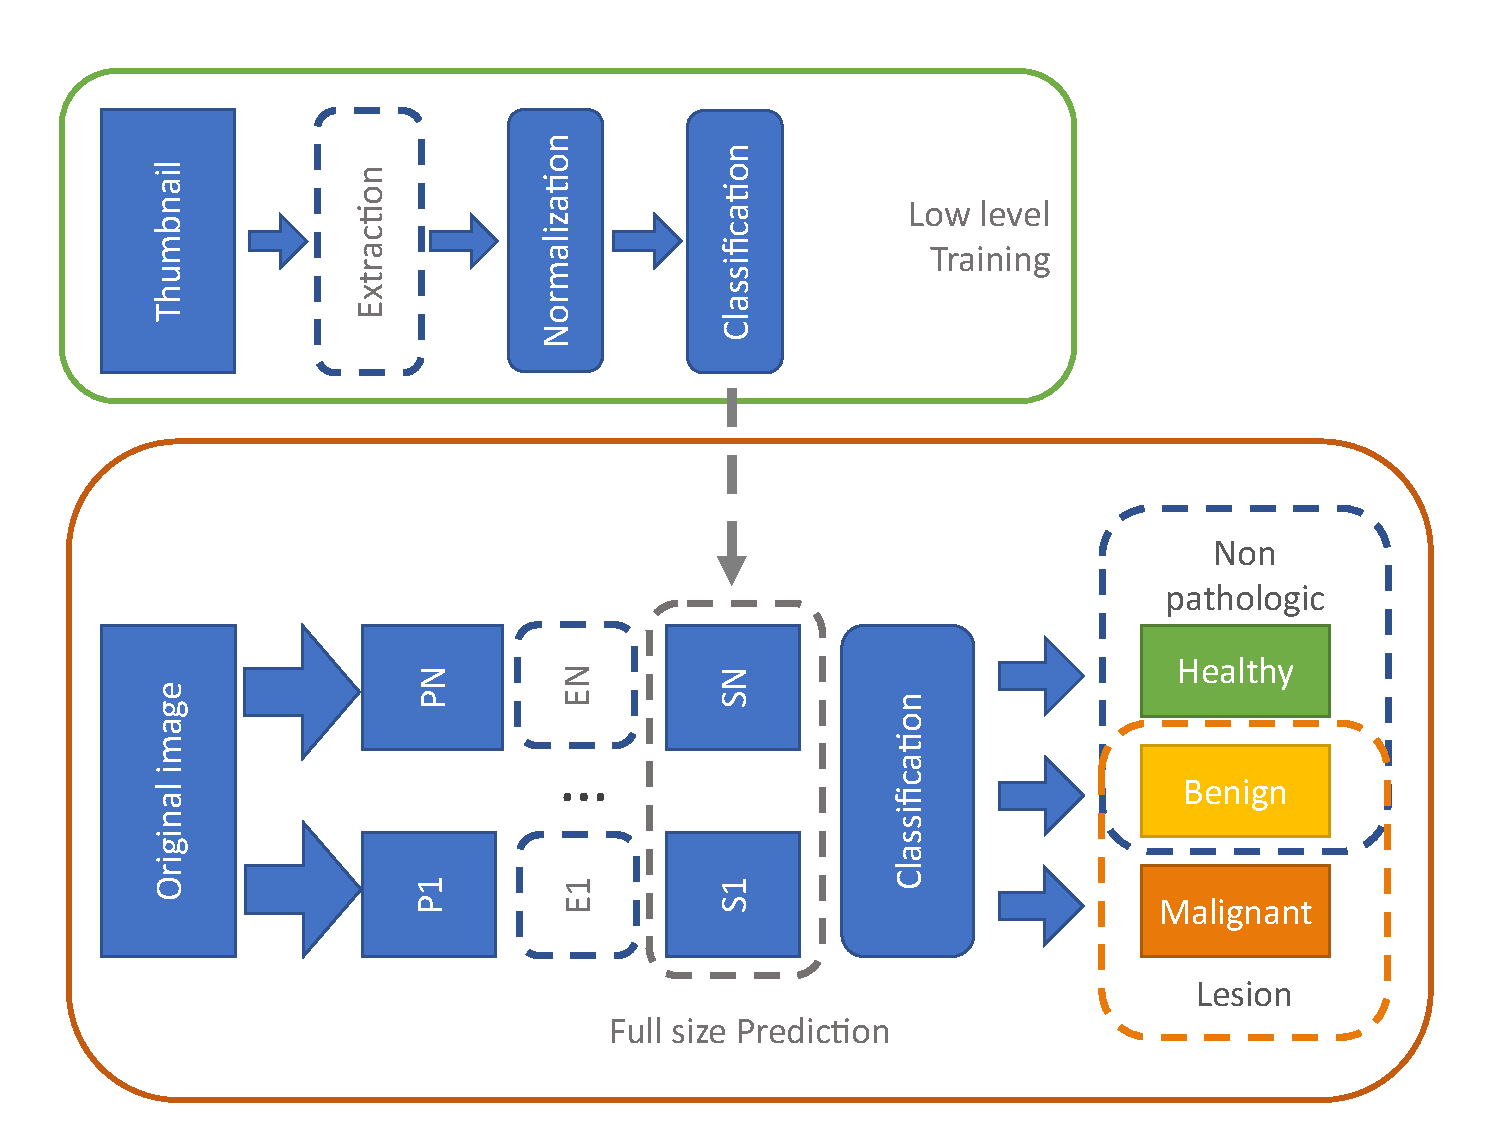
\includegraphics[width=0.65\linewidth]{content/figures/Sliding.pdf}
        \caption{Second pipeline for classification \ac{rcm} images. P1 to PN correspond to Patches, E1 to EN correspond to feature Extraction and S1 to SN correspond to Scores or Decisions obtained for each patches.}
        \label{sliding}
    \end{center} 
\end{figure}
\section{Results and discussion}
\label{results}
We first describe the raw dataset provided by dermatologists and the one we derived from it, which is more appropriate for evaluation and . Then we describe and explain the experiments and describe the obtained results.\par
\subsection{Datasets Description}
All the data we use in this study was provided by dermatology service of Saint-Etienne hospital under patient consent. This data contain three modalities of images: Clinical Photography, Dermatoscopy and \ac{rcm}. Each of these modalities is acquired by a specialist. Furthermore, each patient is associated to a ground truth label from histopathology \cite{Cinotti2018}.\par
In this work, we focus only on the \ac{rcm} images and Lentigo pathology parts of this dataset. Images related to this imaging modality are acquired into the dermoepidermal junction, considered by specialist as relevant for diagnosis of Benign Lentigo and Malignant Lentigo. The depth of acquisition nor the spatial location information are not available. Processed \ac{rcm} images from this dataset have spatial resolution of 1000 by 1000 pixels, with a quantification on a single channel on 1 byte.\par
As our goal is to provide a classification over images, we build a new dataset with an annotation on each image, with the help of a specialist. This dataset contain 2098 \ac{rcm} annotated images related to 60 patients. The same three types of labels as previously have been assigned: “Malignant” label for images including at least malignant information, “Benign” label for images being composed of benign pathology and finally a “Healthy” label corresponding to absence of Malignant and Benign characteristics. In further references, we will consider it as our “Original images”.\par
\begin{figure}[H]
\centering
    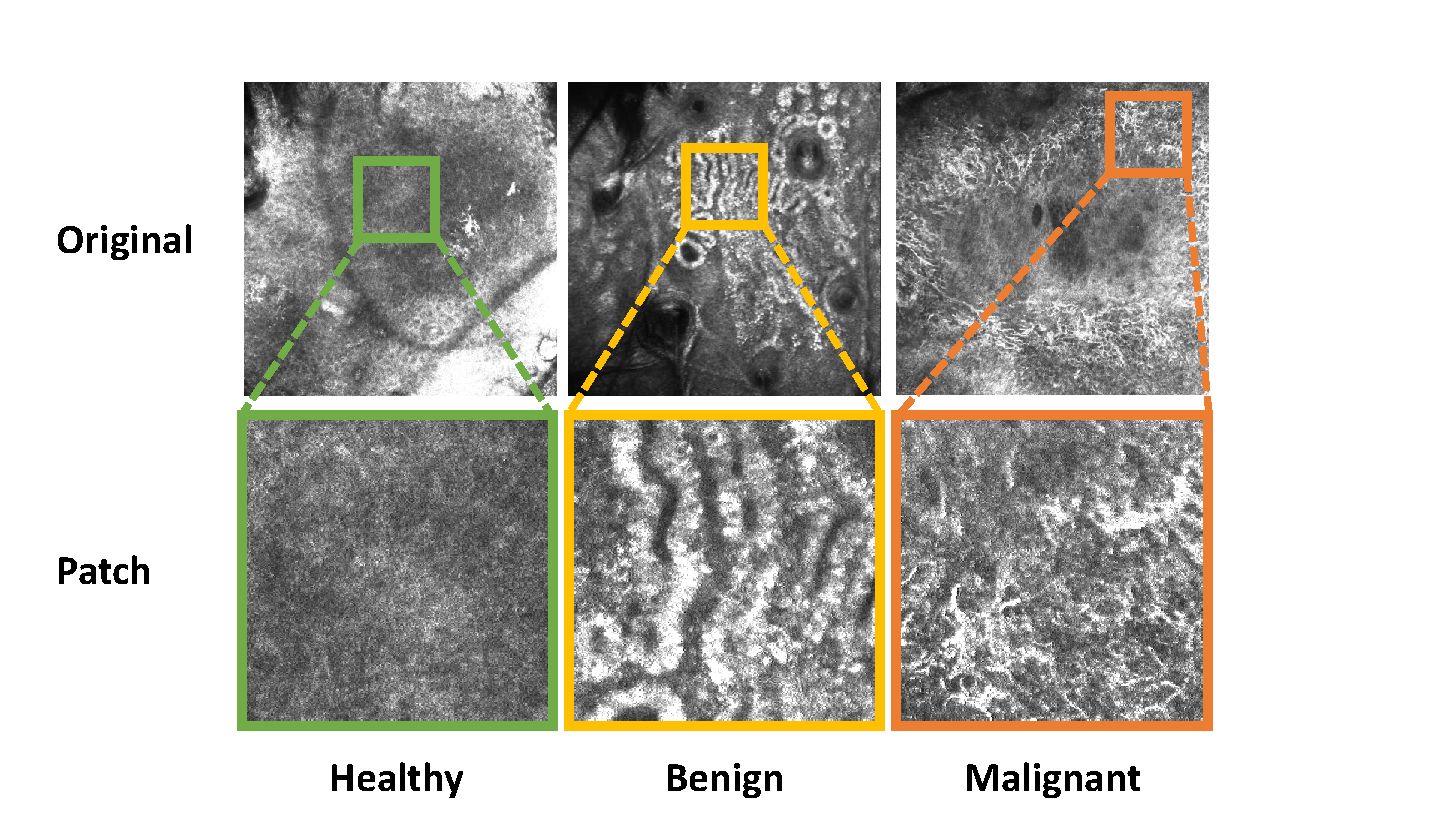
\includegraphics[width=0.9\linewidth]{content/figures/Data.pdf}
    \caption{Examples of full images and extracted patches from skin dermal-epidermal junction with \ac{rcm}.}
    \label{data}
\end{figure}
Despite of these annotations, an image may contain malignant, benign or both tissues. In addition and for this particular work, we built with guidance of a specialist another subset of data containing images with a single type of tissue. These new data consist of thumbnails with a spatial resolution of 250 by 250 pixels. A total of 2307 thumbnails are extracted belonging to the three previous categories, with respectively 259 healthy images, 1622 benign images and 426 malignant images (see \Cref{data} for extraction example). In the next part of this paper, we will make reference to these data as “Thumbnails”.
\subsection{Results and Analysis}
Our validation protocol remains the same for each experiment: a nested cross validation is used, known to be less biased than simple cross validation way \cite{Cawley2010}. This process allows to cross validate hyperparameters and evaluate objectively prediction models. Each of the cross-validation steps is based on K-Fold strategy with k=5 in our case. For this purpose we use of “Scikit Learn” library for Machine Learning classification, validation and metric~\cite{pedregosa2011scikit}.\par
We evaluate our experiments using F1-Score metric, as it is statistically suitable for unbalanced populations and provide information about recall and precision. In addition, a standard deviation is calculated to achieve an analysis of the stability of models along nested cross validation.\par
\begin{table}[h]
\centering
    \begin{tabular*}{\linewidth}{l@{\extracolsep{\fill}}ll}
        \hline
        \textbf{Methods} & \textbf{Original images} & \textbf{Thumbnails}\\
        \hline
        Wavelets & 0.45$\pm$0.07 & 0.59$\pm$0.05\\
        \hline
        Haralick & 0.49$\pm$0.09 & 0.61$\pm$0.07\\
        \hline
        Transfer Learning (Max Pool) & 0.57$\pm$0.04 & \textbf{0.89$\pm$0.03}\\
        \hline
        Transfer Learning (Avg Pool) & \textbf{0.66$\pm$0.04} & \textbf{0.89$\pm$0.03}\\
    \end{tabular*}
    \caption{Comparison of feature extraction methods for three classes classification using F1-Score on original images and thumbnails.}
    \label{simple_scores}
\end{table}
In \Cref{simple_scores}, we first achieve a comparison over the two handcrafted feature extraction methods, and Transfer Learning methods using “Global Maximum Pooling” and “Global Average Pooling”. In both cases when considering the whole image or when using thumbnails, Transfer Learning methods significantly overtake handcrafted methods (largest score for F1-Score and smallest standard deviation value). Inter-comparison of Transfer learning methods show that the results are similar for MAX and AVG pooling for Thumbnails. However,  when using the entire image, Average Pooling performs better than MAX pooling. This result may be explained by the fact that the activation map is not reduced to a single value as it is the case of Max-Pooling. \par
\begin{table}[h]
\centering
    \begin{tabular*}{\linewidth}{l@{\extracolsep{\fill}}lll}
        \hline
        \textbf{Methods} & \textbf{H vs B vs M} & \textbf{H vs L} & \textbf{NM vs M}\\
        \hline
        Decision level& 0.53$\pm$0.04 & 0.69$\pm$0.03 & 0.70$\pm$0.02\\
        \hline
        Decision level + Overlap & 0.59$\pm$0.01 & 0.71$\pm$0.01 & 0.76$\pm$0.02\\
        \hline
        Score level& 0.69$\pm$0.03 & 0.73$\pm$0.02 & 0.82$\pm$0.02\\
        \hline
        Score level + Overlap & \textbf{0.73$\pm$0.03} & \textbf{0.76$\pm$0.02} & \textbf{0.85$\pm$0.02}\\
    \end{tabular*}
    \caption{Comparison of sliding window methods based on decision or prediction scores and impact of an overlap of half of size through decision.}
    \label{sliding_scores}
\end{table}
Since the best results (in \Cref{simple_scores}) are obtained by use of the Transfer Learning with “Global Average Pooling”, we use it as feature extraction method in next experiments. \Cref{sliding_scores}, provide results of second pipeline (using a sliding window as a way to extract patches over the original \ac{rcm} images. We consider also an overlap between thumbnails of half of their size. The scores obtained for patches are merged later to make a decision (see \Cref{detection} example of low level decisions). This table include comparison over three labels classification and binary classification by performing “Healthy” vs “Lesional” (H vs L) and “Non Malignant” vs “Malignant” (NM vs M). Sliding window prediction based on scores is much more efficient than using simple decisions and seems intuitive as we get more information to explain a single label. Also, the use of an overlap slightly improved classification results in both “Decision level” and “Score level”.\par
\begin{figure}[h]
    \begin{center} 
        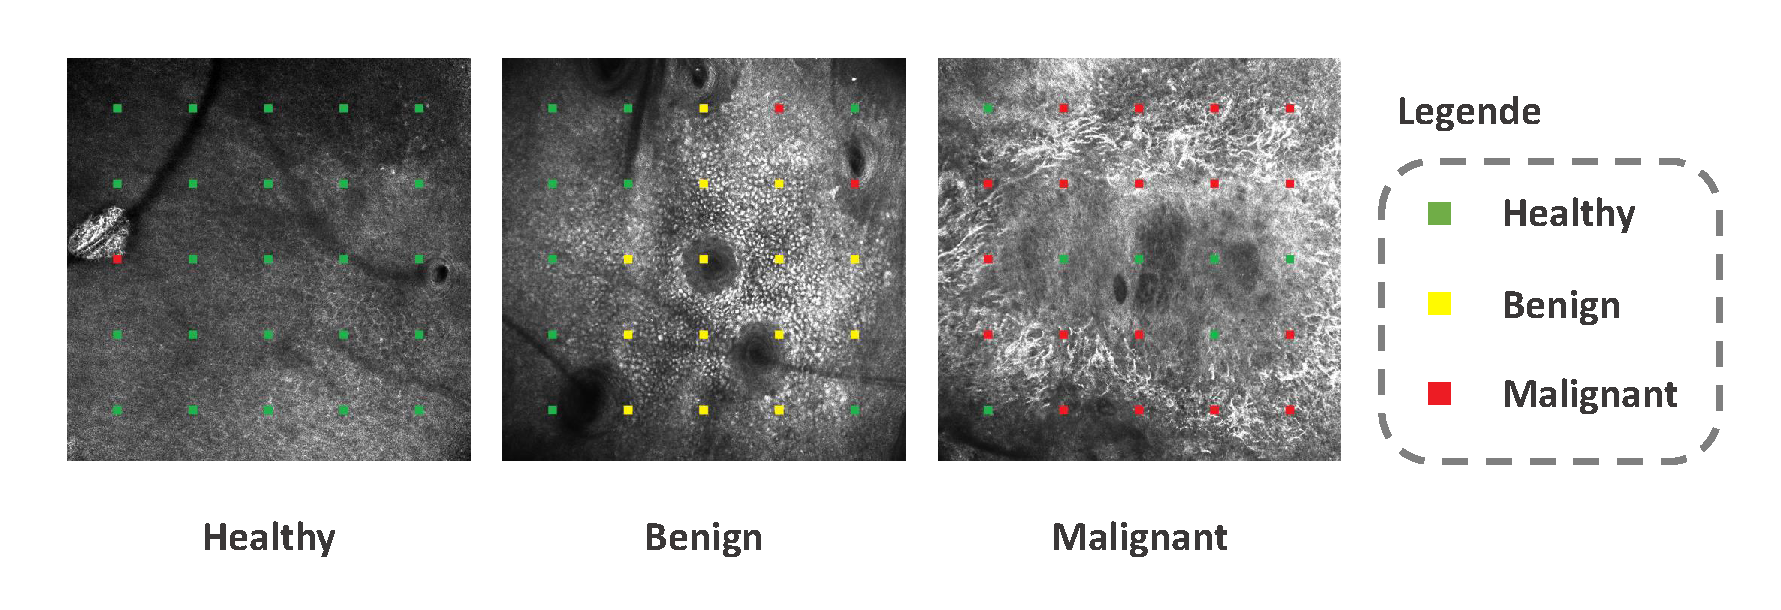
\includegraphics[width=\linewidth]{content/figures/Detection.pdf}
        \caption{Exemple of sliding window performed on full images to reach some local decisions.}
        \label{detection}
    \end{center} 
\end{figure}
Furthermore, this last table shows also that classification of “Non Malignant” against “Malignant” pathologies are much more significant than classification of “Healthy” against “Pathological” and can be due to similarity in patterns between “Healthy” and “Benign” tissues. However, this can be useful in a clinical context as their objectives are to detect malignant pathologies on patients.

\section{Conclusion and Future Work}
\label{conclusion}
In this study, we proposed and evaluated two processing pipelines on \ac{rcm} images for evaluation of Lentigo. These two pipelines exploit in two different ways three approaches for feature extraction, namely Wavelets, Haralick and CNN via Transfer learning. In the first pipeline we operate training and prediction on the whole image wile in the second pipeline a patch-based training and prediction is achieved. The final decision for an image is made by merging the different scores obtained at patch levels. Further research will investigate fine-tuning of last layers as it should give some improvements in this way.\par
Further improvements will consider other ways of merging decisions or score based on existing works to improve existing method.\par

\section*{Aknowledgements}
This research was supported by the Conseil Regional de Bourgogne Franche-Comte, France and the European Regional Development Fund (ERDF).\par
We thank Dr. Perrot and Dr. Cinotti for their work on their dataset and for their permission to use it.\par

{\small
\printbibliography
}

% that's all folks
\end{document}


